% Halloween: trick-or-treating in the USA
% Compile with: latexmk -pdf <file>.tex
\documentclass[aspectratio=169,11pt]{beamer}

\usepackage[T1]{fontenc}
\usepackage{lmodern}
\usepackage{booktabs}
\usepackage{array}
\usepackage{tikz}
\usetikzlibrary{shapes.geometric,positioning,calc,arrows.meta}
\usepackage{pgfplots}
\pgfplotsset{compat=1.18}
\usepackage[most]{tcolorbox}
\graphicspath{{images/}}

% ---------- Colors ----------
\definecolor{navy}{HTML}{1C2541}
\definecolor{oldred}{HTML}{B22234}   % US flag red, also the accent color
\definecolor{oldblue}{HTML}{3C3B6E}  % US flag blue
\definecolor{ink}{HTML}{2B2B2B}
\definecolor{muted}{HTML}{8A8F98}
\definecolor{paper}{HTML}{FFFFFF}
\definecolor{dem}{HTML}{2E5FA3}      % Democrats
\definecolor{rep}{HTML}{C0392B}      % Republicans
\definecolor{austria}{HTML}{C8102E}  % Austria red, for USA-vs-Austria comparisons

% ---------- Minimal theme ----------
\setbeamertemplate{navigation symbols}{}
\setbeamercolor{normal text}{fg=ink, bg=paper}
\setbeamercolor{structure}{fg=navy}
\setbeamercolor{frametitle}{fg=navy}
\setbeamercolor{alerted text}{fg=oldred}
\setbeamercolor{footnote}{fg=muted}
\setbeamerfont{frametitle}{size=\Large, series=\bfseries}
\setbeamertemplate{itemize item}{\color{oldred}\textbullet}
\setbeamertemplate{itemize subitem}{\color{muted}--}
\setbeamertemplate{enumerate item}{\color{oldred}\insertenumlabel.}
\setbeamersize{text margin left=1.1cm, text margin right=1.1cm}
\hypersetup{colorlinks=true, urlcolor=dem, linkcolor=navy}

\setbeamertemplate{frametitle}{%
  \vspace*{0.5cm}%
  \usebeamerfont{frametitle}\usebeamercolor[fg]{frametitle}\insertframetitle\par
  \vspace{0.15cm}{\color{navy!15}\rule{\textwidth}{0.4pt}}\par}

\setbeamertemplate{footline}{%
  \hfill{\tiny\color{muted}\insertframenumber}\hspace*{0.6cm}\vspace*{0.35cm}}

% Plain divider at the start of each section
\AtBeginSection{%
  \begin{frame}[plain,noframenumbering]
    \centering
    {\LARGE\bfseries\color{navy}\insertsection}\\[0.6em]
    {\color{oldred}\rule{1.5cm}{0.8pt}}
  \end{frame}}

% "Think" question slides: \begin{thinkframe} ... \end{thinkframe}
\newenvironment{thinkframe}{%
  \begin{frame}[plain,noframenumbering,environment=thinkframe]\centering\Large}{\end{frame}}

% ---------- Helpers ----------
% Small grey source line at the bottom of a frame
\newcommand{\source}[1]{%
  \begin{tikzpicture}[remember picture,overlay]
    \node[anchor=south west, font=\tiny, text=muted, text width=0.85\paperwidth, align=left]
      at ($(current page.south west)+(0.6cm,0.25cm)$) {#1};
  \end{tikzpicture}}

% Quote box with a thin red rule on the left; optional arg e.g. [fontupper=\itshape\small]
\newtcolorbox{textquote}[1][]{%
  enhanced, frame hidden, boxrule=0pt, sharp corners,
  colback=navy!4, borderline west={2pt}{0pt}{oldred},
  left=10pt, right=8pt, top=6pt, bottom=6pt, fontupper=\itshape, #1}

% Photo + name + short bio (use inside a column): \candidate{file}{Name}{bio}
\newcommand{\candidate}[3]{%
  \begin{minipage}[t]{\linewidth}\centering
    \includegraphics[height=3.5cm]{#1}\\[0.5em]
    {\large\bfseries\color{navy}#2}\\[0.4em]
    \begin{minipage}{0.9\linewidth}\raggedright\small #3\end{minipage}
  \end{minipage}}

% Big number with a caption (use inside a column): \bignum{color}{91\%}{caption}
\newcommand{\bignum}[3]{%
  \begin{minipage}[t]{\linewidth}\centering
    {\fontsize{34}{38}\selectfont\bfseries\color{#1}#2}\\[0.3em]
    {\small #3}
  \end{minipage}}

% US flag drawn in TikZ (hoist height = #1), e.g. \usflag{3cm}
\newcommand{\usflag}[1]{%
  \begin{tikzpicture}[x=#1, y=#1]
    \def\fly{1.9}
    \foreach \i in {0,...,12} {
      \pgfmathsetmacro{\c}{mod(\i,2)==0 ? 1 : 0}
      \ifdim\c pt=1pt
        \fill[oldred] (0,{1-(\i+1)/13}) rectangle (\fly,{1-\i/13});
      \else
        \fill[white] (0,{1-(\i+1)/13}) rectangle (\fly,{1-\i/13});
      \fi
    }
    \def\cw{0.76} \def\ch{0.5385}
    \fill[oldblue] (0,{1-\ch}) rectangle (\cw,1);
    \foreach \r in {1,...,9} {
      \pgfmathsetmacro{\isodd}{mod(\r,2)}
      \ifdim\isodd pt=1pt
        \foreach \k in {0,...,5}
          \node[star, star points=5, star point ratio=2.618, fill=white, inner sep=0pt,
                minimum size=0.0616*#1] at ({(2*\k+1)*\cw/12},{1-\r*\ch/10}) {};
      \else
        \foreach \k in {0,...,4}
          \node[star, star points=5, star point ratio=2.618, fill=white, inner sep=0pt,
                minimum size=0.0616*#1] at ({(2*\k+2)*\cw/12},{1-\r*\ch/10}) {};
      \fi
    }
    \draw[ink!30, line width=0.3pt] (0,0) rectangle (\fly,1);
  \end{tikzpicture}}

% Agree/disagree spectrum for "spectrum game" activities
\newcommand{\spectrum}{%
  
\begin{tikzpicture}
    \shade[left color=oldblue, right color=oldred, rounded corners=2pt] (0,0) rectangle (11,0.18);
    \node[anchor=north, font=\small, text=oldblue] at (0,-0.15) {Strongly disagree};
    \node[anchor=north, font=\small, text=muted] at (5.5,-0.15) {Neutral};
    \node[anchor=north, font=\small, text=oldred] at (11,-0.15) {Strongly agree};
    \fill[paper, draw=muted] (5.5,0.09) circle (2.5pt);
  \end{tikzpicture}}

% One statement per slide: \statement{number}{total}{text}
\newcommand{\statement}[3]{%
  \begin{frame}[plain]
    \vfill
    \begin{center}
      {\small\color{muted}Statement #1 of #2}\\[1.2em]
      {\LARGE\bfseries #3}
    \end{center}
    \vfill
    \begin{center}\spectrum\end{center}
    \vspace{1.2cm}
  \end{frame}}


% One myth-or-fact slide: \mythfact{statement}{photo}{credit}{FACT/MYTH}{color}{explanation}
\newcommand{\mythfact}[6]{%
  \begin{frame}{Myth or fact?}
    \begin{columns}[c]
      \begin{column}{0.5\textwidth}
        {\LARGE\bfseries\color{navy} #1}
        \vspace{1.5em}

        \uncover<2>{%
          {\Large\bfseries\color{#5} #4}\\[0.6em]
          {\normalsize #6}}
      \end{column}
      \begin{column}{0.45\textwidth}
        \centering
        \includegraphics[width=\linewidth, height=5.6cm, keepaspectratio]{#2}\\[0.2em]
        {\tiny\color{muted} #3\par}
      \end{column}
    \end{columns}
  \end{frame}}

% Text on the left, one photo on the right: \photoslide{title}{photo}{credit}{content}
\newcommand{\photoslide}[4]{%
  \begin{frame}{#1}
    \begin{columns}[c]
      \begin{column}{0.52\textwidth}
        #4
      \end{column}
      \begin{column}{0.44\textwidth}
        \centering
        \includegraphics[width=\linewidth, height=5.8cm, keepaspectratio]{#2}\\[0.2em]
        {\tiny\color{muted} #3\par}
      \end{column}
    \end{columns}
  \end{frame}}

\definecolor{orange}{HTML}{D35400}
\definecolor{fact}{HTML}{2E7D32}

\begin{document}

% ---------- Title slide ----------
\begin{frame}[plain]
  \begin{columns}[c]
    \begin{column}{0.55\textwidth}
      {\fontsize{30}{34}\selectfont\bfseries\color{navy} Halloween}\\[0.8em]
      {\Large\color{muted} Trick-or-treating in the USA}\\[0.6em]
      {\color{orange}\rule{3cm}{1.5pt}}
    \end{column}
    \begin{column}{0.4\textwidth}
      \centering
      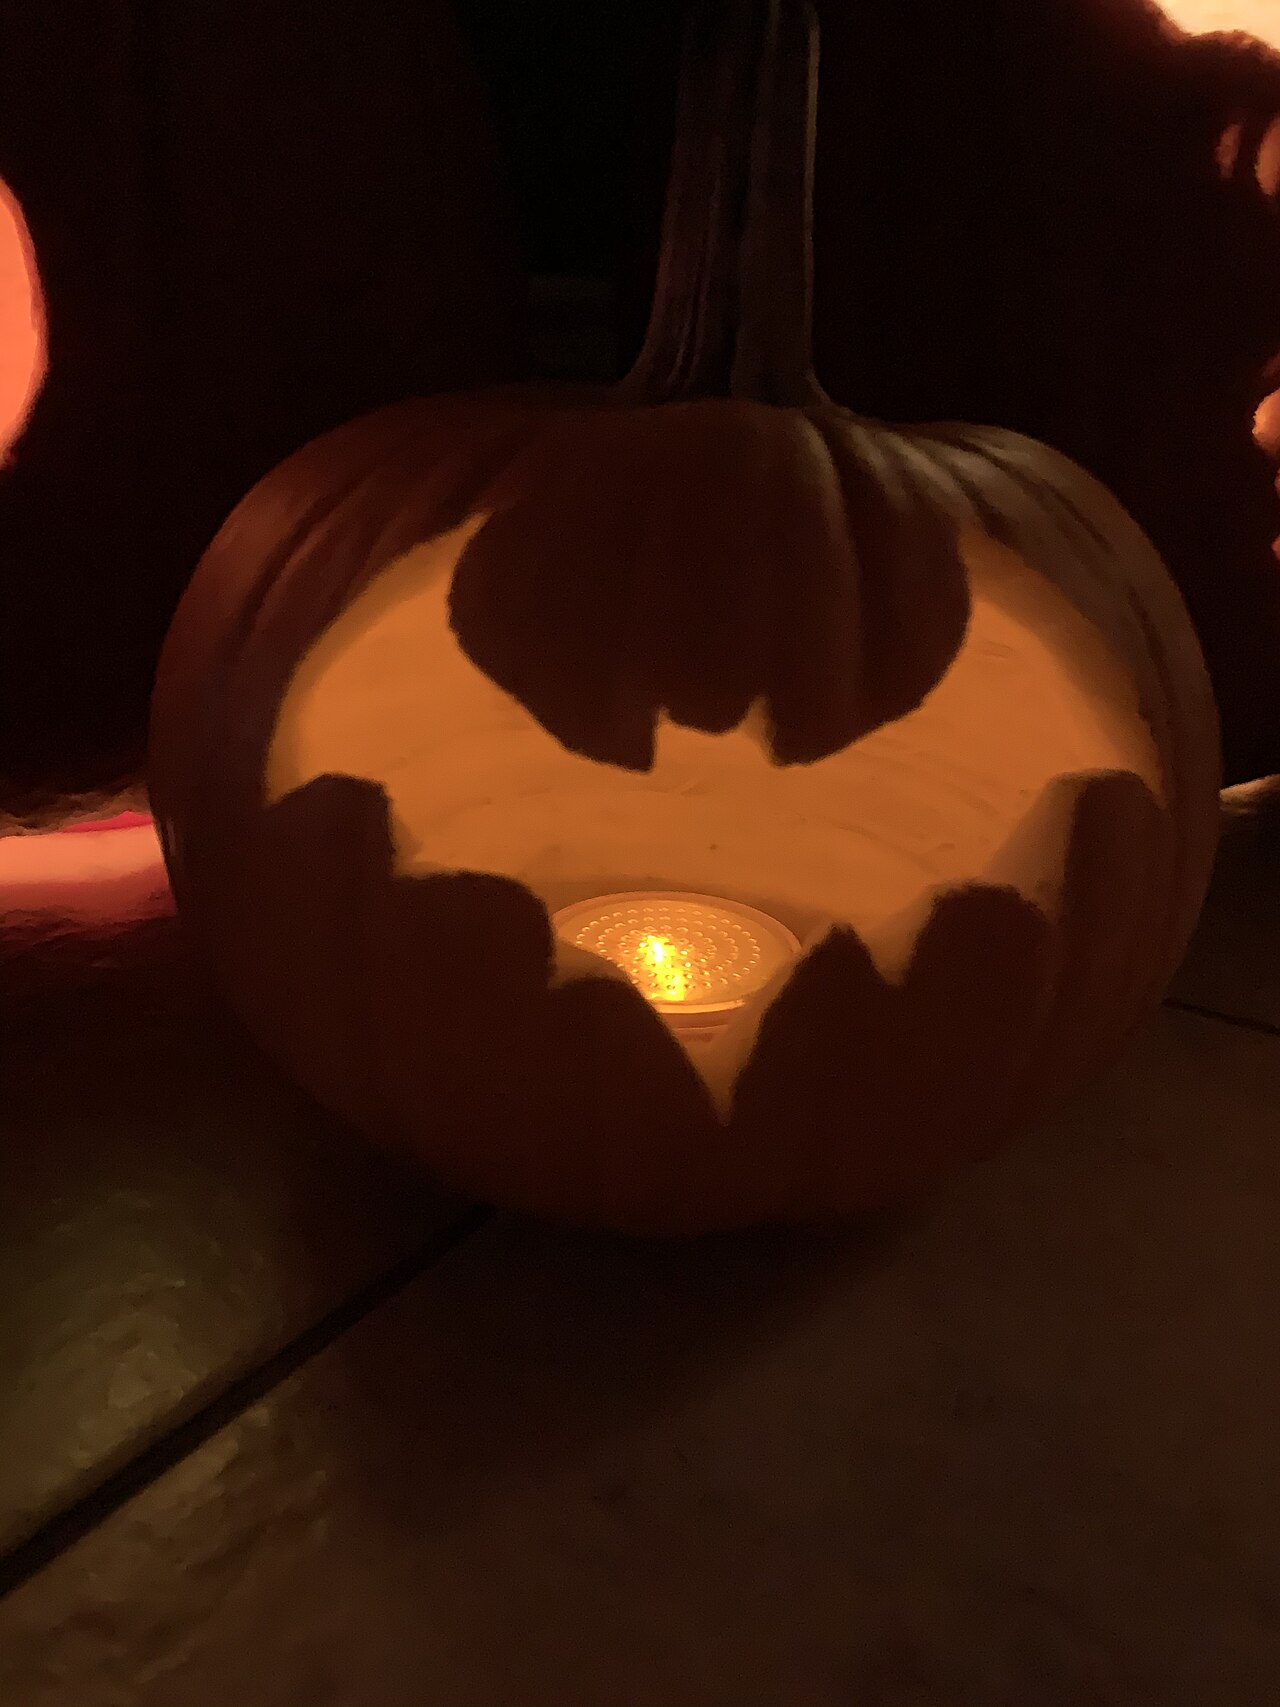
\includegraphics[height=6.2cm]{jol36.jpg}\\[0.2em]
      {\tiny\color{muted} Photo: LostplanetKD73, CC BY-SA 4.0\par}
    \end{column}
  \end{columns}
\end{frame}

% =====================================================================
\section{Warm-up}

\photoslide{Warm-up}{candy_bowl.jpg}{Photo: U.S.\ Air Force}{%
  {\Large What do you know about Halloween and trick-or-treating?}
  \vspace{1.2em}

  \color{muted} Go around the room: everyone says one thing.}

% =====================================================================
\section{A Brief History}

\photoslide{Ancient Greece}{swallows.jpg}{Swallows in a Greek wall painting from Akrotiri. Photo: Zde, CC BY-SA 4.0}{%
  \begin{itemize}\setlength{\itemsep}{1em}
    \item The writer \textbf{Athenaeus of Naucratis} (lived around AD 200) describes a custom on the island of Rhodes
    \item Children dressed up as \alert{swallows}
    \item They went door to door singing a song and asking for food
  \end{itemize}}

\photoslide{No food? Mischief!}{swallows.jpg}{Swallows in a Greek wall painting from Akrotiri. Photo: Zde, CC BY-SA 4.0}{%
  \begin{itemize}\setlength{\itemsep}{1em}
    \item If the owner of a house gave them nothing, the children threatened \alert{mischief}
    \item The song even threatens to carry off the front door!
    \item Does this sound familiar?
  \end{itemize}}

\photoslide{16th-century Scotland: guising}{guisers.jpg}{Halloween guisers in Shetland, Scotland. Photo: Mike Pennington, CC BY-SA 2.0}{%
  \begin{itemize}\setlength{\itemsep}{1em}
    \item In Scotland, Halloween was the time for \alert{guising}
    \item \textbf{Etymology:} what do you think this word means?
  \end{itemize}
  \vspace{0.8em}
  \uncover<2>{%
    \begin{itemize}\setlength{\itemsep}{0.6em}
      \item From \emph{guise} = appearance, as in \emph{disguise}
      \item Same Germanic root as German \emph{Weise} (\emph{Art und Weise})
    \end{itemize}}}

\photoslide{What is guising?}{turnip.jpg}{A traditional Scottish turnip lantern (``tumshie''). Photo: LornaMCampbell, CC BY-SA 4.0}{%
  \begin{itemize}\setlength{\itemsep}{1em}
    \item Children go \alert{door to door in disguise}
    \item They perform a song, a poem or a joke
    \item In return they get gifts: apples, nuts, sweets or coins
    \item The first ``jack-o'-lanterns'' were carved \alert{turnips}, not pumpkins
  \end{itemize}}

\photoslide{The roots: Samhain}{bonfire.jpg}{A Samhain bonfire in Ireland. Photo: EWilson, CC BY-SA 4.0}{%
  \begin{itemize}\setlength{\itemsep}{1em}
    \item Guising goes back to the Celtic festival of \emph{Samhain} (October 31--November 1), the start of winter
    \item People believed the spirits of the dead came into the human world
    \item They dressed up \alert{as spirits} for protection, and received gifts in their name
  \end{itemize}}

\begin{frame}{Guising comes to North America}
  \centering
  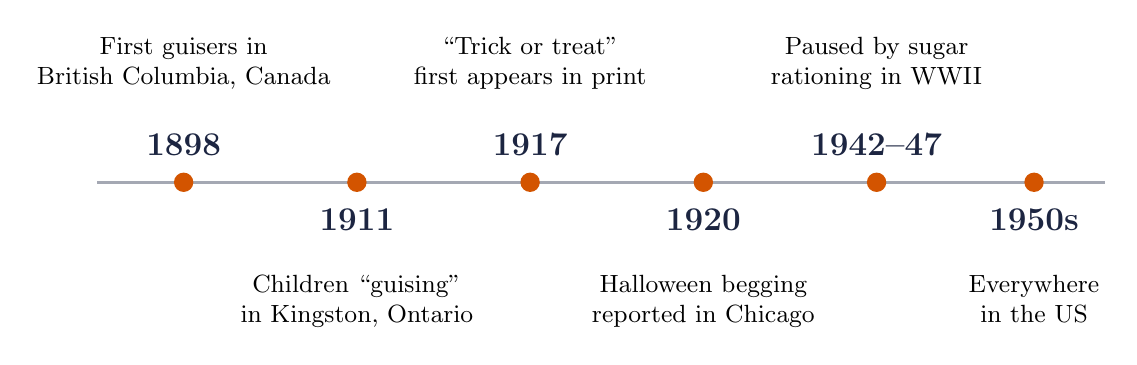
\begin{tikzpicture}[x=1cm, y=1cm]
    \draw[navy!40, line width=1.2pt] (-0.2,0) -- (12.6,0);
    \foreach \x in {0.9, 3.1, 5.3, 7.5, 9.7, 11.7} \fill[orange] (\x,0) circle (3.5pt);
    \node[font=\bfseries\large, text=navy, above=6pt] at (0.9,0) {1898};
    \node[font=\small, align=center, above=30pt] at (0.9,0) {First guisers in\\British Columbia, Canada};
    \node[font=\bfseries\large, text=navy, below=6pt] at (3.1,0) {1911};
    \node[font=\small, align=center, below=30pt] at (3.1,0) {Children ``guising''\\in Kingston, Ontario};
    \node[font=\bfseries\large, text=navy, above=6pt] at (5.3,0) {1917};
    \node[font=\small, align=center, above=30pt] at (5.3,0) {``Trick or treat''\\first appears in print};
    \node[font=\bfseries\large, text=navy, below=6pt] at (7.5,0) {1920};
    \node[font=\small, align=center, below=30pt] at (7.5,0) {Halloween begging\\reported in Chicago};
    \node[font=\bfseries\large, text=navy, above=6pt] at (9.7,0) {1942--47};
    \node[font=\small, align=center, above=30pt] at (9.7,0) {Paused by sugar\\rationing in WWII};
    \node[font=\bfseries\large, text=navy, below=6pt] at (11.7,0) {1950s};
    \node[font=\small, align=center, below=30pt] at (11.7,0) {Everywhere\\in the US};
  \end{tikzpicture}
\end{frame}

\begin{frame}{Before Halloween: Ragamuffin Day}
  \begin{columns}[c]
    \begin{column}{0.4\textwidth}
      \begin{itemize}\setlength{\itemsep}{1em}
        \item From 1870 to the 1930s, begging from strangers happened on \alert{Thanksgiving}, not Halloween
        \item In New York City, children dressed up as beggars: \emph{Ragamuffin Day}
      \end{itemize}
    \end{column}
    \begin{column}{0.56\textwidth}
      \centering
      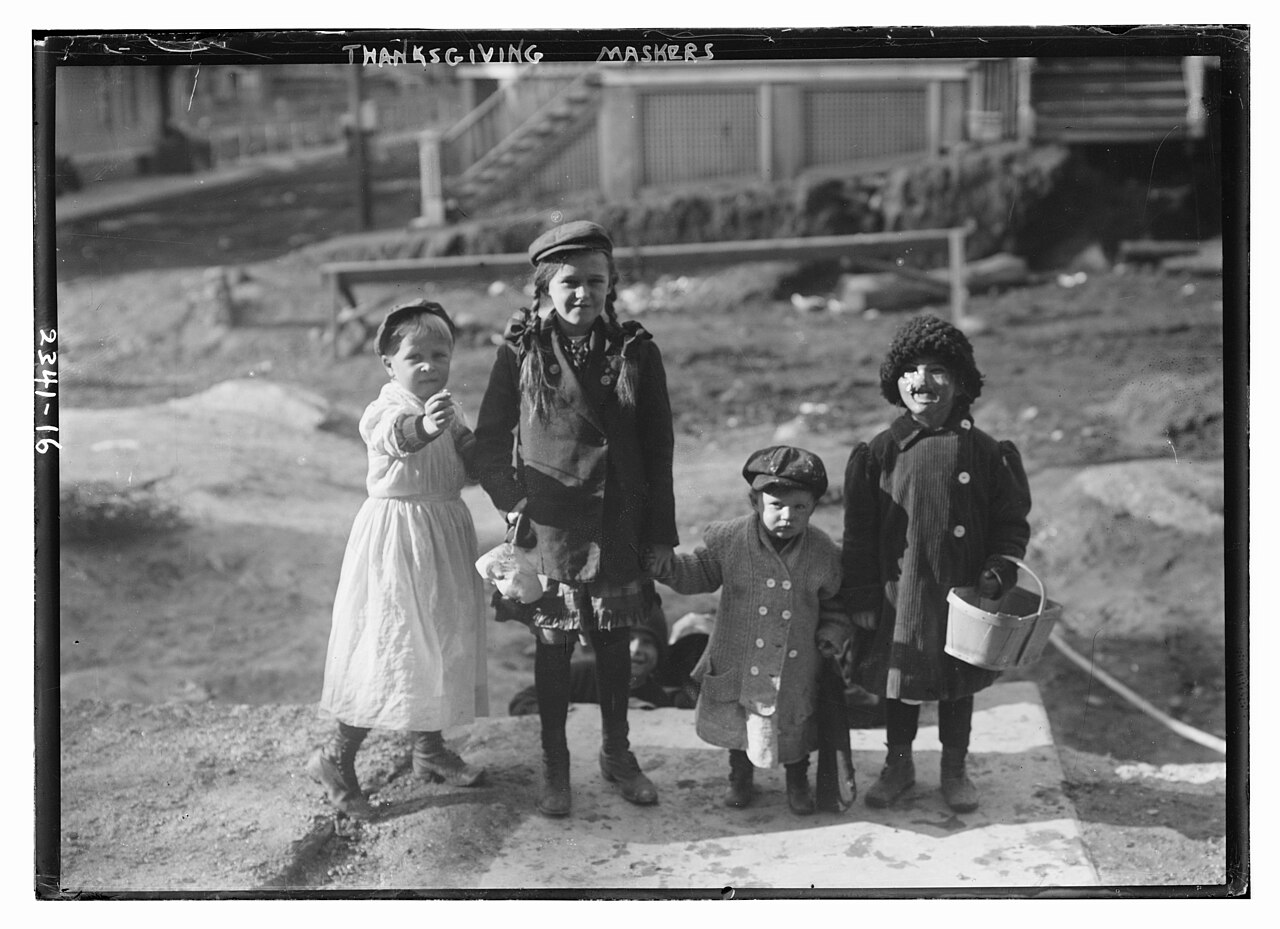
\includegraphics[width=0.49\linewidth]{ragamuffins1.jpg}\hfill
      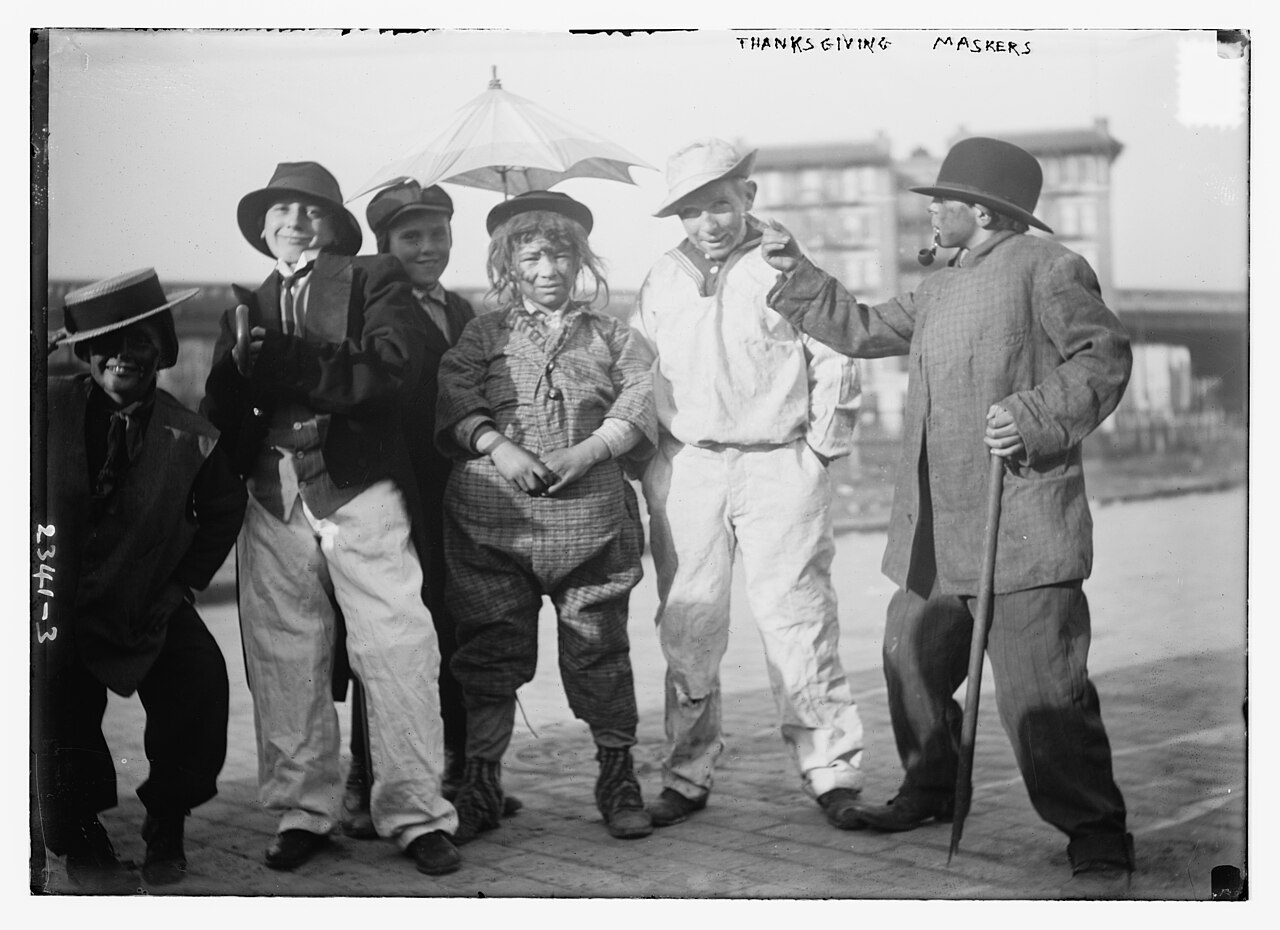
\includegraphics[width=0.49\linewidth]{ragamuffins2.jpg}\\[0.2em]
      {\tiny\color{muted} ``Thanksgiving maskers'' in New York, 1910s. Photos: Bain News Service, Library of Congress\par}
    \end{column}
  \end{columns}
\end{frame}

\photoslide{Trick-or-treating takes off}{party1935.jpg}{Children at a Halloween party, Los Angeles, 1935. Photo: Los Angeles Times, CC BY 4.0}{%
  \begin{itemize}\setlength{\itemsep}{1em}
    \item In the 1920s and 30s, trick-or-treating became more and more popular
    \item Halloween parties for children spread too
  \end{itemize}}

\photoslide{A pause for World War II}{rationing.jpg}{Food rationing in the US during World War II. Photo: U.S.\ Office of War Information}{%
  \begin{itemize}\setlength{\itemsep}{1em}
    \item From 1942 to 1947, \alert{sugar was rationed}: no sugar, no candy
    \item Trick-or-treating paused
    \item After the war it came back bigger than ever, helped by radio shows, comics like \emph{Peanuts}, and Disney cartoons
  \end{itemize}}

% =====================================================================
\section{What Do We Actually Do?}

\begin{frame}{Halloween in numbers}
  \vfill
  \begin{columns}[T]
    \begin{column}{0.3\textwidth}
      \bignum{orange}{74\%}{of Americans celebrate Halloween}
    \end{column}
    \begin{column}{0.3\textwidth}
      \bignum{orange}{61\%}{hand out candy}
    \end{column}
    \begin{column}{0.3\textwidth}
      \bignum{orange}{\$13.5B}{total spending, a new record\\(\$4.1 billion just on candy)}
    \end{column}
  \end{columns}
  \vfill
  \source{Source: National Retail Federation, Halloween survey (September 2026).}
\end{frame}

\begin{frame}{A caveat: New York is different}
  \centering
  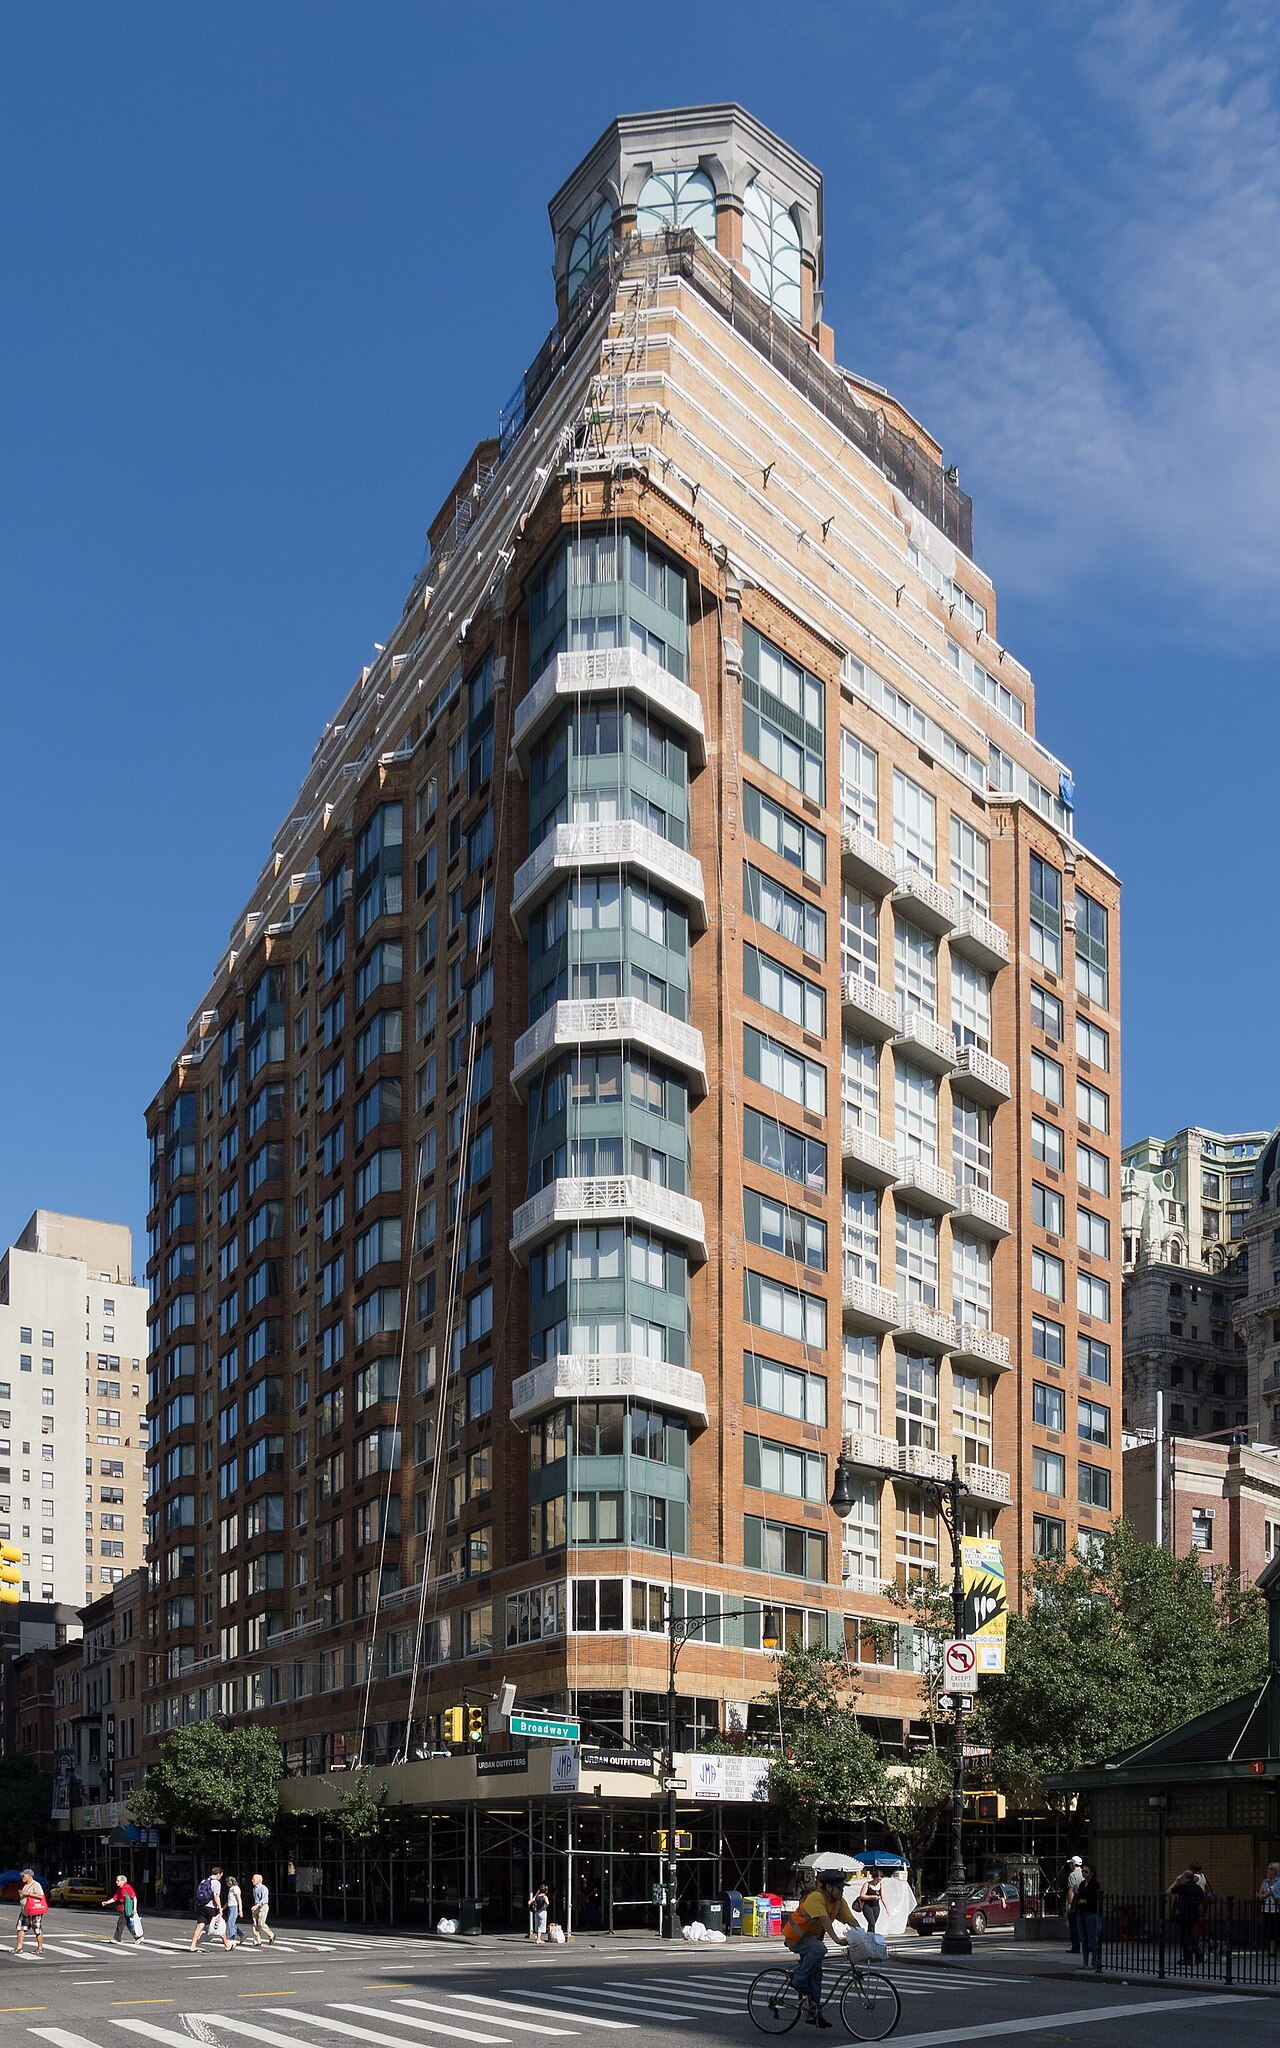
\includegraphics[height=5.6cm]{highrise.jpg}\hspace{0.6cm}%
  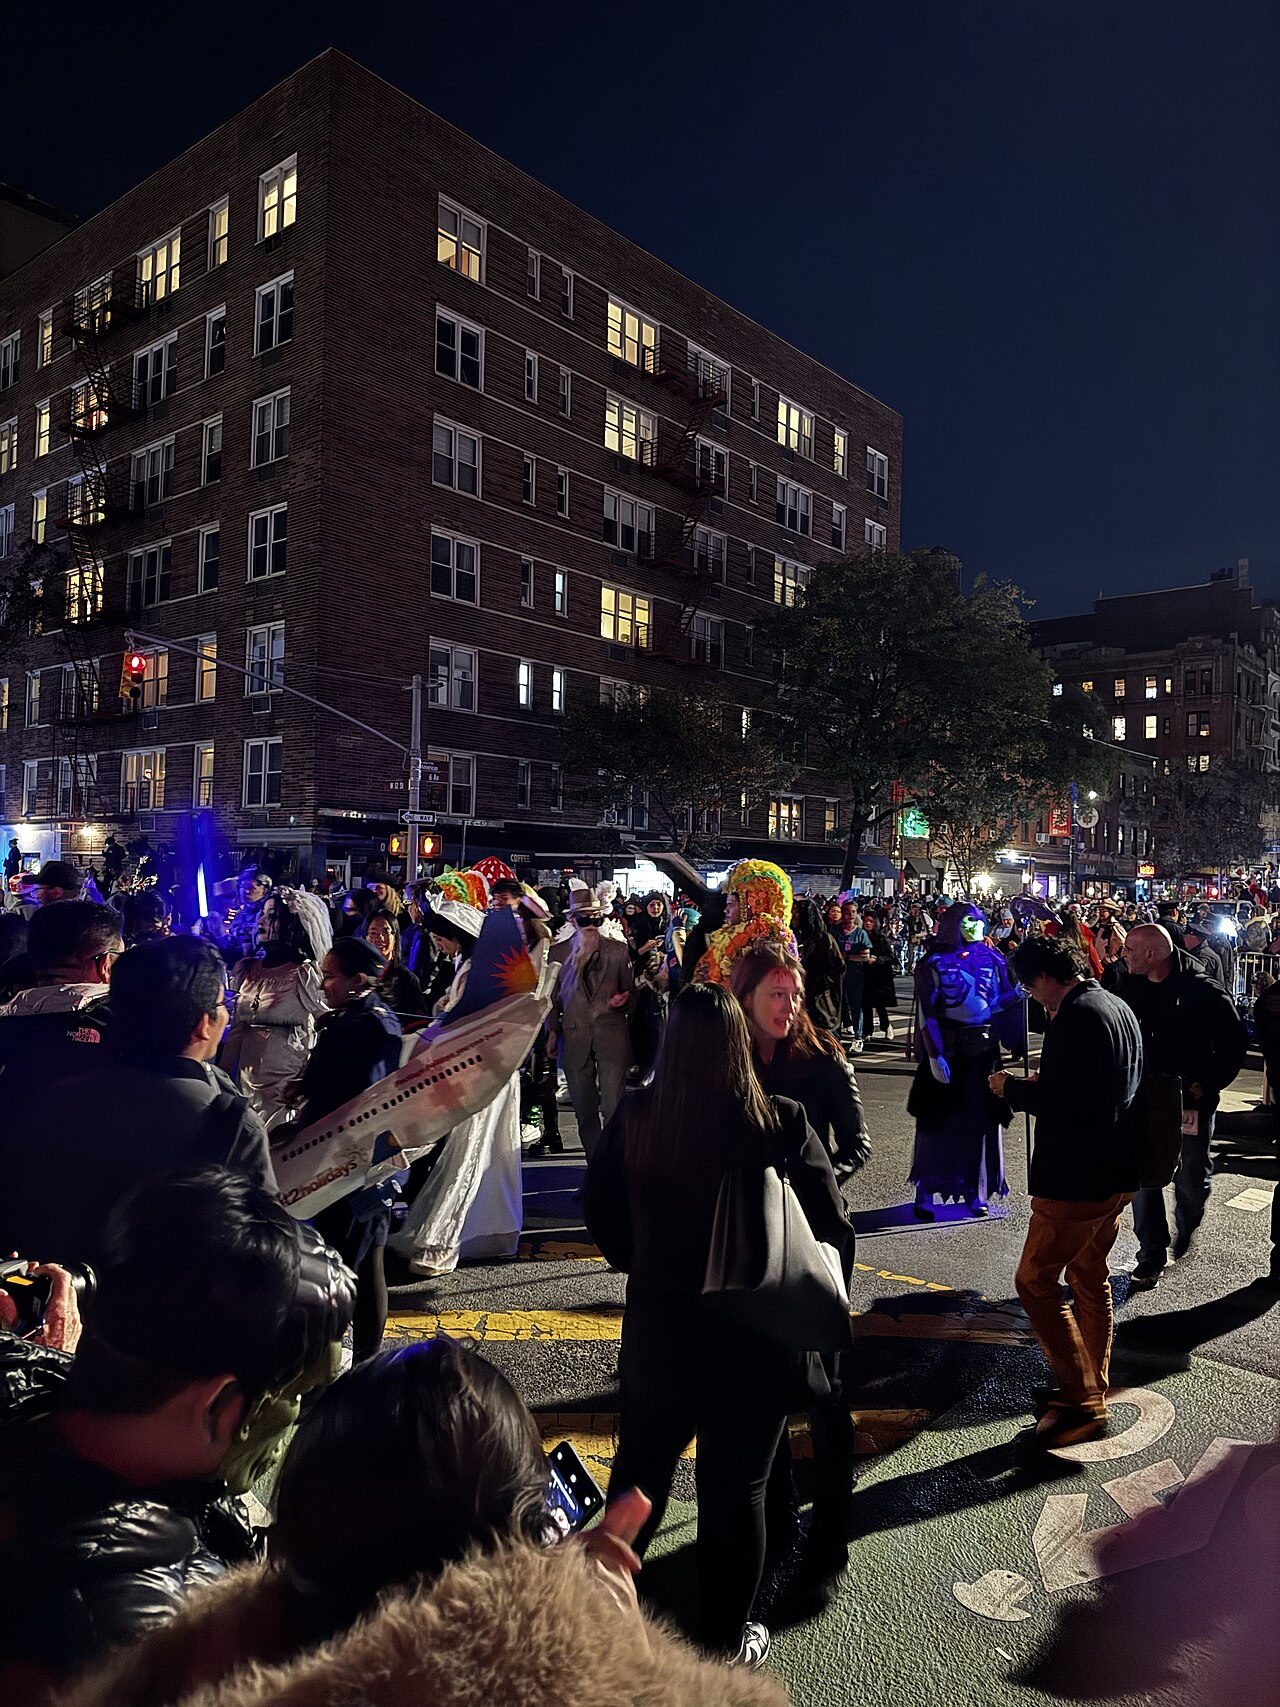
\includegraphics[height=5.6cm]{parade.jpg}\\[0.3em]
  {\tiny\color{muted} Left: an apartment building on the Upper West Side (King of Hearts, CC BY-SA 4.0). Right: the Village Halloween Parade, Manhattan (Tzim78, CC BY 4.0)\par}
\end{frame}

\subsection{Myth vs.\ Fact}

\begin{frame}{Myth vs.\ fact}
  \centering
  {\LARGE Which of these traditions do we \alert{actually} do on Halloween?}
  \vspace{1.5em}

  {\large\color{muted} Guess: myth or fact?}
\end{frame}

\mythfact{1.\ Wear costumes}{skeleton_kid.jpg}{Photo: Don Scarborough, CC BY-SA 2.5}{FACT}{fact}{Almost every child dresses up.}

\mythfact{2.\ Go to many different buildings}{door.jpg}{Photo: Belinda Hankins Miller, CC BY 2.0}{MYTH}{oldred}{In New York you stay in your own building and go from apartment to apartment.}

\mythfact{3.\ Say the full rhyme: ``Trick or treat, smell my feet, give me something good to eat!''}{dublin.jpg}{Photo: Sarah777, public domain}{MYTH}{oldred}{We just say ``Trick or treat!''}

\mythfact{4.\ TP (toilet paper) people's houses}{tp_house.jpg}{Photo: Jackie from Monmouth County, NJ, CC BY 2.0}{MYTH}{oldred}{Mostly a teenage prank, and rare.}

\subsection{Things We Do}

\begin{frame}{Goal: as much candy as possible}
  \begin{columns}[c]
    \begin{column}{0.48\textwidth}
      \begin{itemize}\setlength{\itemsep}{1em}
        \item Many buildings post a \alert{sign-up sheet} in the lobby
        \item Neighbors who want trick-or-treaters write down their apartment
        \item Start at the \alert{top} of the building and work your way down
      \end{itemize}
    \end{column}
    \begin{column}{0.46\textwidth}
      \centering
      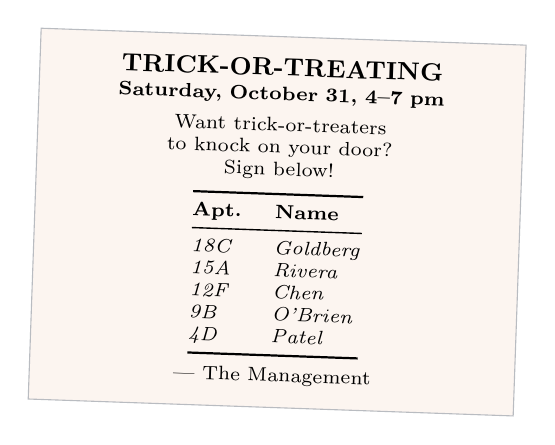
\begin{tikzpicture}
        \node[draw=muted!60, fill=orange!6, inner sep=8pt, rotate=-2, text width=5.6cm, align=center, font=\scriptsize] {%
          {\small\bfseries TRICK-OR-TREATING}\\[0.1em]
          {\bfseries Saturday, October 31, 4--7 pm}\\[0.4em]
          Want trick-or-treaters to knock on your door?\\
          Sign below!\\[0.5em]
          \begin{tabular}{@{}ll@{}}
            \toprule
            \textbf{Apt.} & \textbf{Name} \\
            \midrule
            \textit{18C} & \textit{Goldberg} \\
            \textit{15A} & \textit{Rivera} \\
            \textit{12F} & \textit{Chen} \\
            \textit{9B} & \textit{O'Brien} \\
            \textit{4D} & \textit{Patel} \\
            \bottomrule
          \end{tabular}\\[0.4em]
          --- The Management};
      \end{tikzpicture}\\[0.4em]
      {\tiny\color{muted} A recreation of a typical lobby sign-up sheet\par}
    \end{column}
  \end{columns}
\end{frame}

\photoslide{Pro tips}{highrise.jpg}{Photo: King of Hearts, CC BY-SA 4.0}{%
  \begin{itemize}\setlength{\itemsep}{1em}
    \item The \alert{biggest} buildings (high-rises) are usually the best: more apartments, more candy
    \item Shops on the street also give out candy
    \item Forget the little bucket: bring a \alert{large pillowcase}
  \end{itemize}}

\photoslide{Pumpkin carving}{carving.jpg}{Photo: Bobjgalindo, CC BY 4.0}{%
  \begin{itemize}\setlength{\itemsep}{1em}
    \item Before Halloween, families carve pumpkins into \alert{jack-o'-lanterns}
    \item A candle goes inside
    \item Remember: in Scotland and Ireland they used turnips!
  \end{itemize}}

\begin{frame}{After trick-or-treating}
  \begin{itemize}\setlength{\itemsep}{1.2em}\large
    \item Empty the pillowcase onto the floor
    \pause
    \item Trade candy with siblings and friends
    \pause
    \item Eat the candy
    \pause
    \item \alert{Feel sick}
  \end{itemize}
\end{frame}

\subsection{Things We Don't Do}

\photoslide{Things we don't do: tricks}{tp_house.jpg}{Photo: Jackie from Monmouth County, NJ, CC BY 2.0}{%
  \begin{itemize}\setlength{\itemsep}{1em}
    \item Nobody does the \alert{``trick''} part of trick-or-treat
    \item If a house has no candy, you just go to the next one
  \end{itemize}}

\photoslide{Things we don't do: go building to building}{brownstones.jpg}{Brownstones in Park Slope, Brooklyn. Photo: Danny Lyon, public domain}{%
  \begin{itemize}\setlength{\itemsep}{1em}
    \item In New York you usually stay \alert{inside your own building}
    \item The exception: \alert{brownstone} neighborhoods in Brooklyn, where people decorate their stoops and kids go house to house
    \item \href{https://www.instagram.com/p/DeUcz-WETzg/}{See what that looks like}
  \end{itemize}}

\photoslide{Things we don't do: elaborate costumes}{globe_costume.jpg}{Photo: MatadorianGray, CC BY 3.0}{%
  \begin{itemize}\setlength{\itemsep}{1em}
    \item Most people buy a simple costume or make one at home
    \item Only a few people go all out
    \item \ldots like this
  \end{itemize}}

\subsection{After the Age of 16}

\begin{frame}{After the age of 16}
  \begin{itemize}\setlength{\itemsep}{1.2em}\large
    \item Nobody goes trick-or-treating anymore
    \item Instead: \alert{Halloween parties}
    \item Usually pretty \alert{cringe}
  \end{itemize}
\end{frame}

\begin{frame}{The lazy costume}
  \begin{columns}[c]
    \begin{column}{0.3\textwidth}
      \begin{itemize}\setlength{\itemsep}{1em}
        \item Costumes get \alert{lazier} with age
        \item Cat ears + black clothes = a cat
        \item A T-shirt + antennae = a bee
      \end{itemize}
    \end{column}
    \begin{column}{0.66\textwidth}
      \centering
      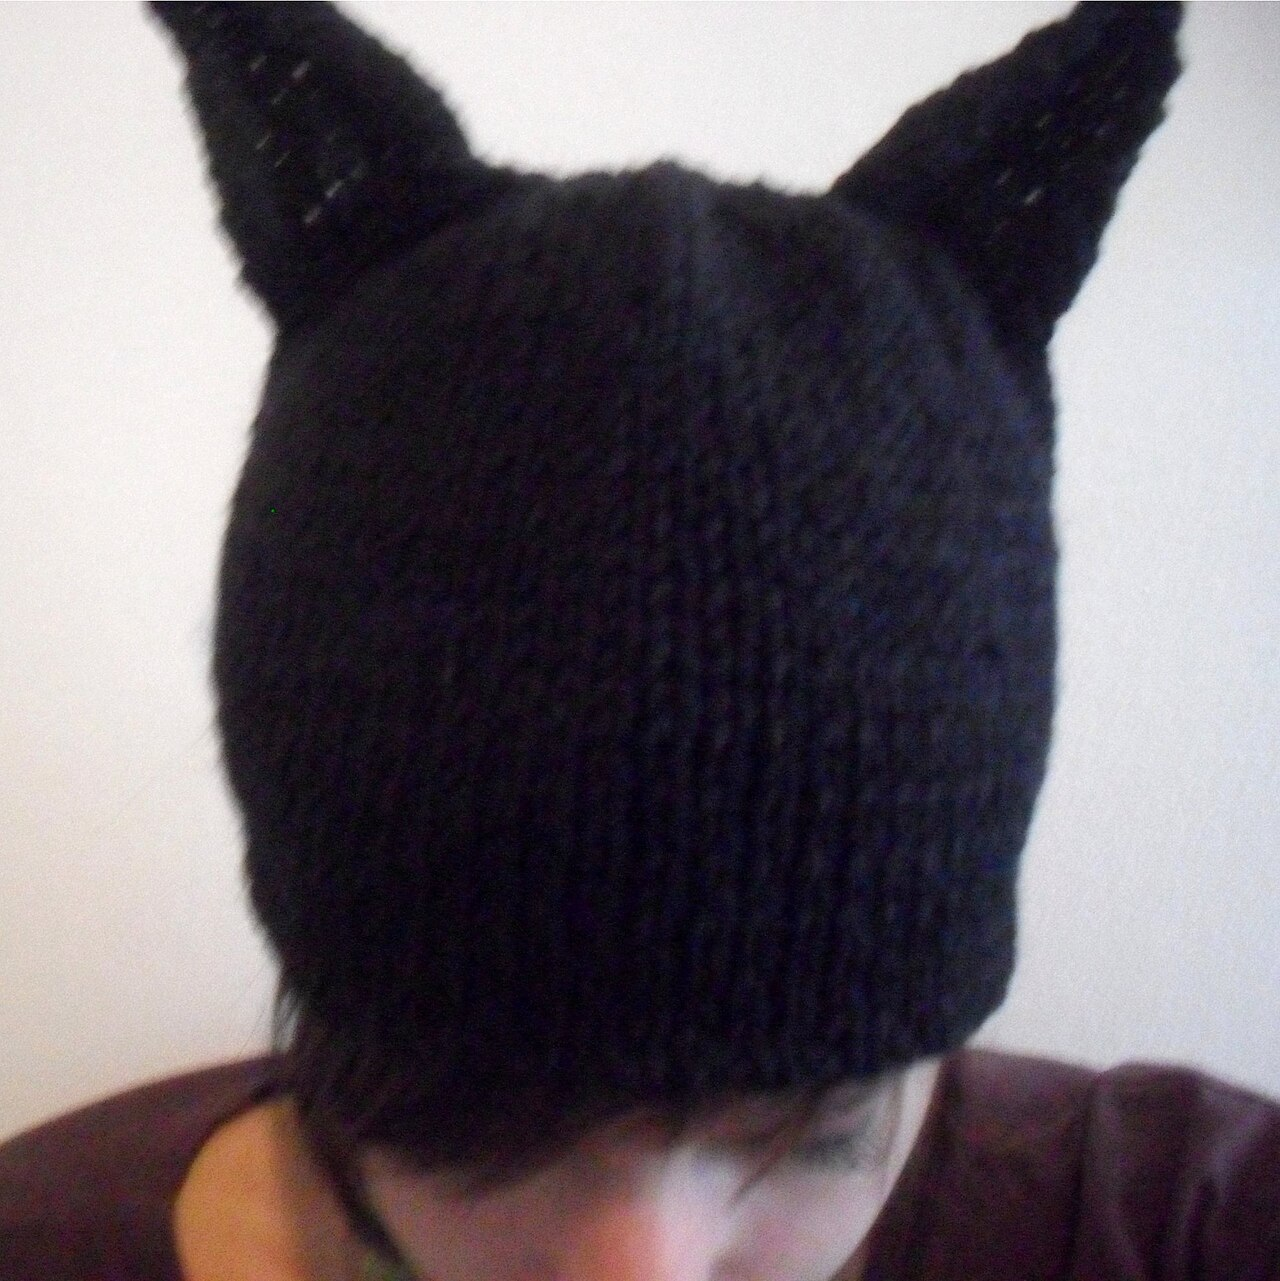
\includegraphics[width=0.48\linewidth, height=4.6cm, keepaspectratio]{cat_hat.jpg}\hfill
      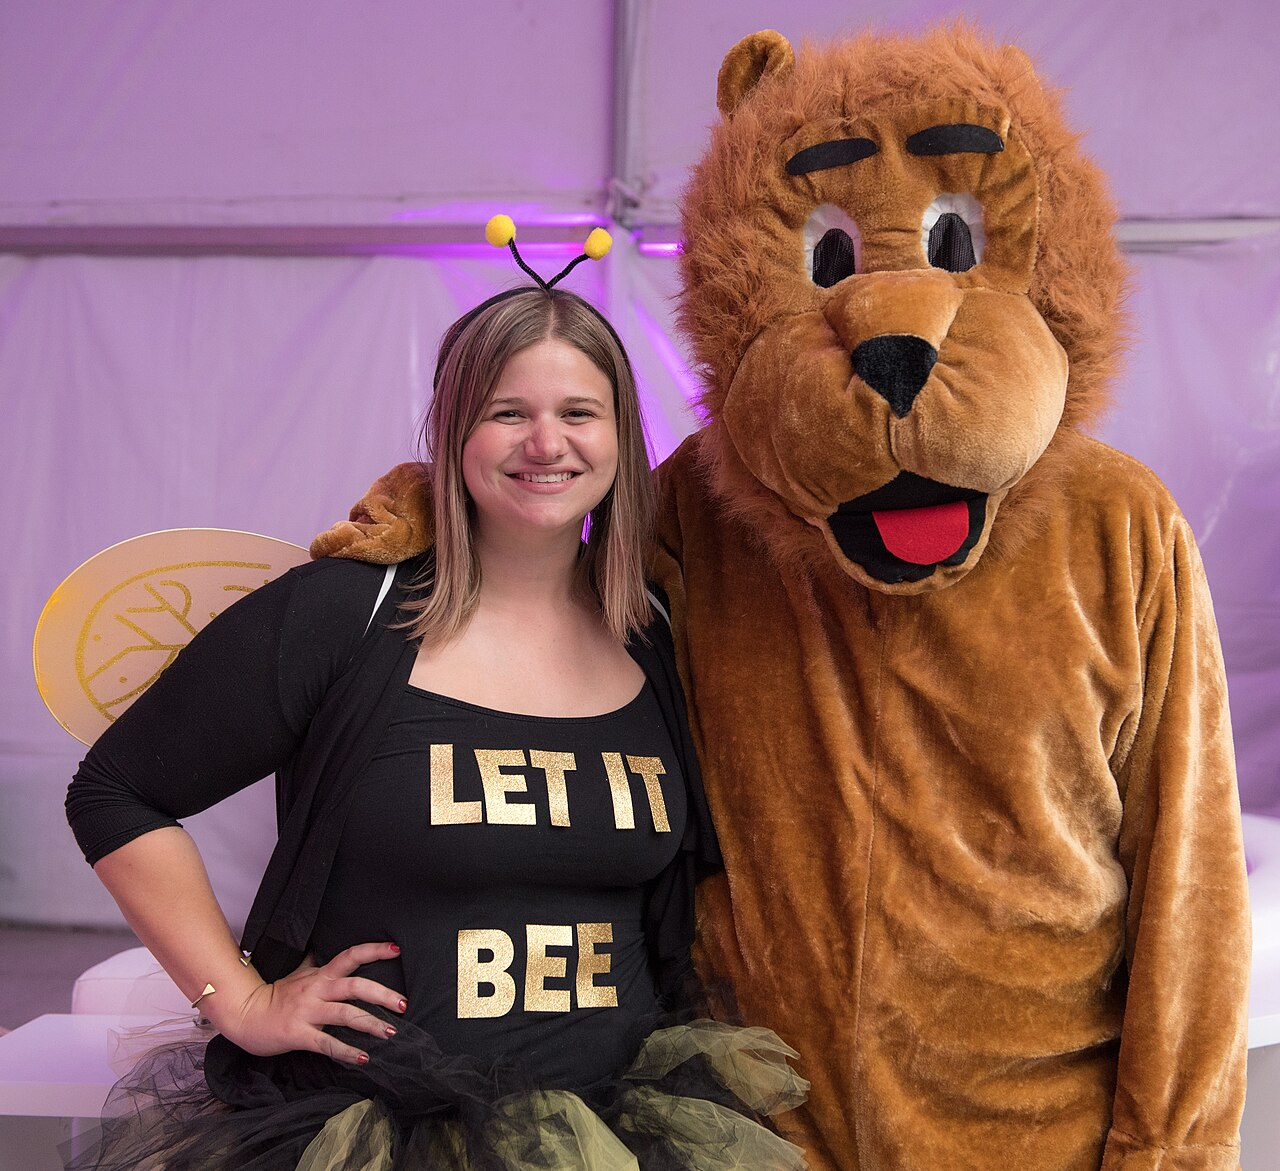
\includegraphics[width=0.48\linewidth, height=4.6cm, keepaspectratio]{let_it_bee.jpg}\\[0.2em]
      {\tiny\color{muted} Left: Annie Pilon, CC BY 2.0. Right: a lazy bee next to a not-so-lazy lion, LBJ Library, public domain\par}
    \end{column}
  \end{columns}
\end{frame}

% =====================================================================
\section{Activity}

\photoslide{Guess the costumes}{witch.jpg}{Photo: Petr Kratochvil, CC0}{%
  \relax{\Large What are the \alert{top 5} costumes in the US this year?}
  \vspace{1.2em}
  \begin{itemize}\setlength{\itemsep}{0.8em}
    \item For children
    \item For adults
    \item Bonus: for pets!
  \end{itemize}}

\begin{frame}{The answers: top costumes of 2026}
  \centering
  \renewcommand{\arraystretch}{1.35}
  \begin{tabular}{@{}cll@{\hspace{1.5cm}}ll@{}}
    \toprule
    & \textbf{\color{orange}Children} & & \textbf{\color{orange}Adults} & \\
    \midrule
    1 & Spider-Man & \color{muted}4.6 million & Witch & \color{muted}4.8 million \\
    2 & Superhero & \color{muted}2.3 million & Vampire & \color{muted}4.2 million \\
    3 & Princess & \color{muted}2.2 million & Batman & \color{muted}2.0 million \\
    4 & Witch & \color{muted}1.6 million & Spider-Man & \color{muted}1.5 million \\
    5 & Ghost & \color{muted}1.6 million & Ghost & \color{muted}1.4 million \\
    \bottomrule
  \end{tabular}

  \vspace{1.2em}
  \textbf{Pets:} 1.\ Pumpkin \quad 2.\ Hot dog \quad 3.\ Ghost
  \source{Source: National Retail Federation, Halloween survey (September 2026).}
\end{frame}

\begin{frame}{And in Austria?}
  \begin{columns}[T]
    \begin{column}{0.48\textwidth}
      \centering
      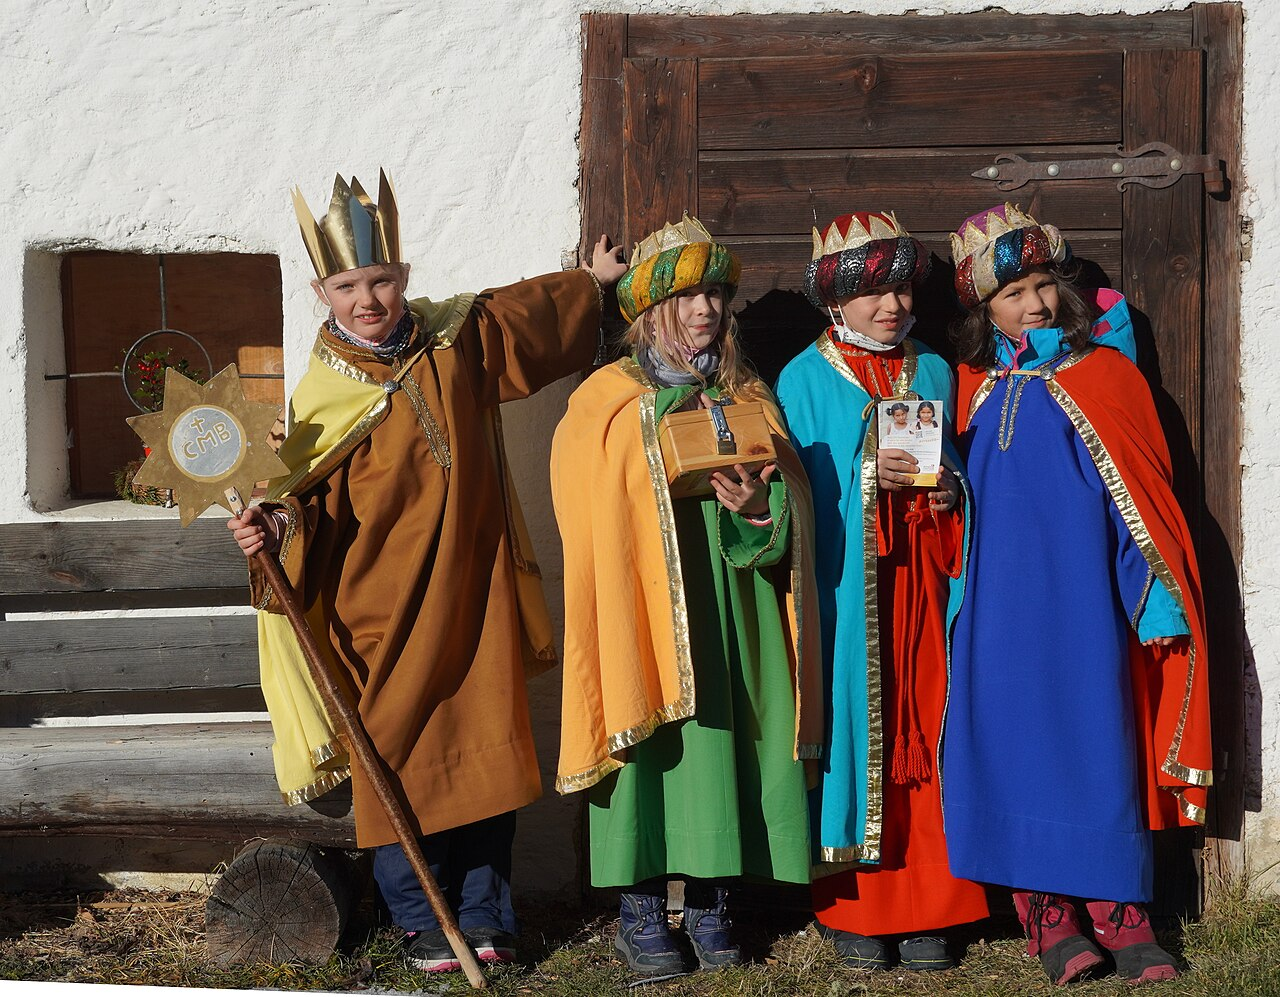
\includegraphics[height=3.6cm]{sternsinger.jpg}\\[0.2em]
      {\tiny\color{muted} Sternsinger in Carinthia. Photo: Naturpuur, CC BY 4.0\par}
      \vspace{0.4em}
      \raggedright\small \textbf{Sternsinger} (January): children in costume go door to door, sing, and collect money
    \end{column}
    \begin{column}{0.48\textwidth}
      \centering
      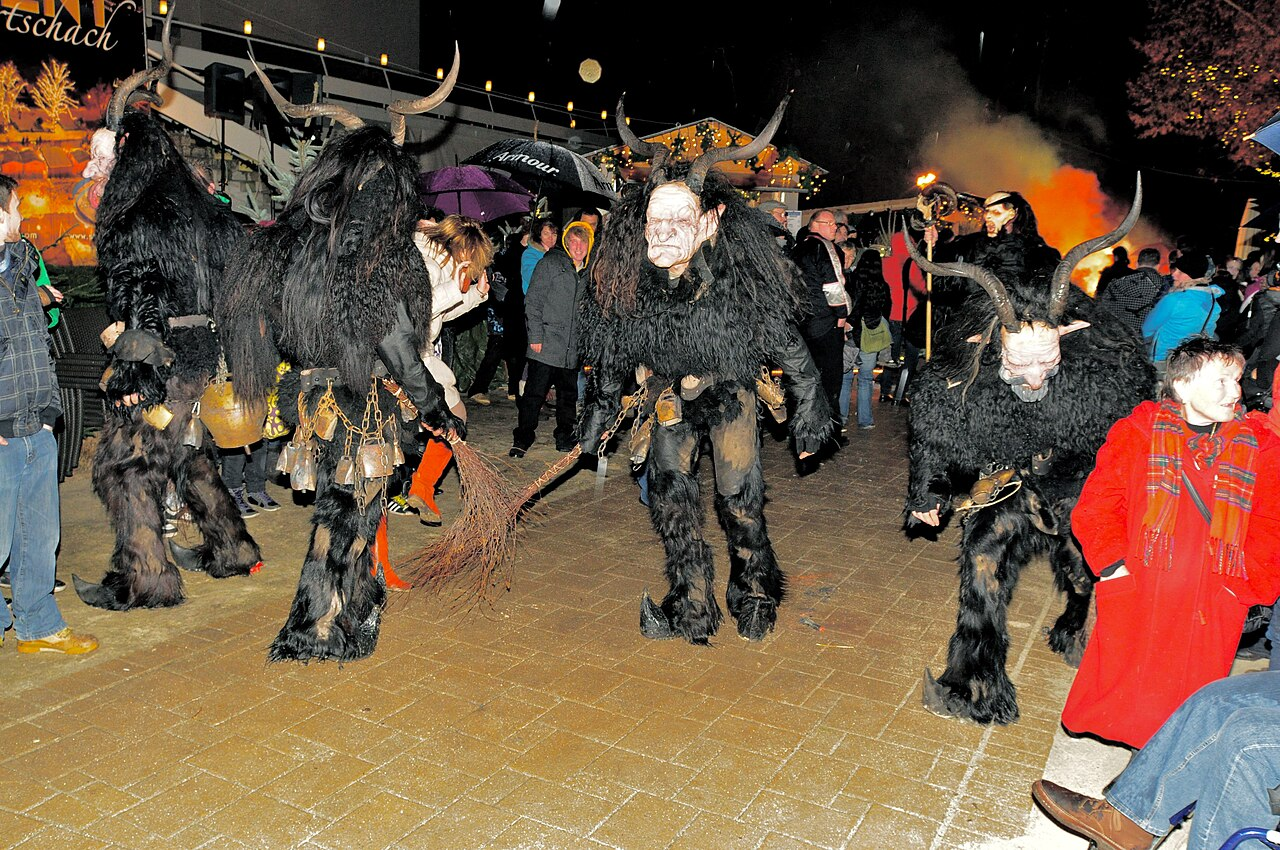
\includegraphics[height=3.6cm]{krampus.jpg}\\[0.2em]
      {\tiny\color{muted} Krampuslauf in Pörtschach. Photo: Johann Jaritz, CC BY-SA 3.0 AT\par}
      \vspace{0.4em}
      \raggedright\small \textbf{Krampus} (December): scary costumes in the streets
    \end{column}
  \end{columns}
  \vfill
  \centering\alert{Which is closest to American Halloween?}
\end{frame}

\begin{frame}[plain,noframenumbering]
  \centering
  {\LARGE\bfseries\color{navy} Happy Halloween!}\\[0.6em]
  {\color{orange}\rule{1.5cm}{0.8pt}}
\end{frame}

\end{document}
